%=============================================================
% Chapitre 5 — Modélisation Machine Learning
%=============================================================
\chapter{Modélisation par Machine Learning}
\label{ch:ml}

\section{Chargement du jeu de données depuis MongoDB}

La première étape du pipeline ML consiste à charger la collection \texttt{data\_final}
directement depuis \textbf{MongoDB}, sans passer par aucun fichier intermédiaire :

\begin{verbatim}
from pymongo import MongoClient
import pandas as pd

db = MongoClient("mongodb://localhost:27017/")["electio_analytics"]
df = pd.DataFrame(list(db["data_final"].find({}, {"_id": 0})))

X = df.drop(columns=["label"])
y = df["label"]
print(f"Jeu de données : {df.shape[0]} observations x {df.shape[1]} colonnes")
# -> Jeu de données : 40000 observations x 171 colonnes
\end{verbatim}

\section{Configuration expérimentale}

\subsection{Split train/test}

Le jeu de données (40 000 observations) est divisé en :
\begin{itemize}
  \item \textbf{Entraînement} : 32 000 observations (80\%), stratifié par classe
  \item \textbf{Test} : 8 000 observations (20\%), stratifié par classe
\end{itemize}

La stratification garantit que chaque split respecte la distribution originale des
classes (10/20/40/20/10\%).

\subsection{Protocole de validation}

Chaque modèle est évalué par \textbf{validation croisée 5-fold} sur le jeu d'entraînement,
puis évalué une fois sur le jeu de test (score final). Les métriques retenues sont :
\begin{itemize}
  \item \textbf{Accuracy} : proportion de prédictions correctes
  \item \textbf{F1-score macro} : moyenne des F1 par classe (pénalise les déséquilibres)
\end{itemize}

\section{Cinq algorithmes testés}

\begin{table}[H]
\centering
\caption{Comparaison des 5 modèles ML — métriques finales (jeu de test, 8 000 obs.)}
\label{tab:model_comparison}
\begin{tabular}{lrrrr}
\toprule
\textbf{Modèle} & \textbf{CV Accuracy} & \textbf{Test Accuracy} & \textbf{F1 Macro} & \textbf{Rang} \\
\midrule
\rowcolor{green!15}
\textbf{HistGradientBoosting} & \textbf{82,11\%} & \textbf{82,11\%} & \textbf{82,10\%} & \textbf{1\textsuperscript{er}} \\
LogisticRegression  & 82,08\% & 82,08\% & 82,04\% & 2\textsuperscript{e} \\
XGBoost             & 82,05\% & 82,05\% & 82,03\% & 3\textsuperscript{e} \\
RandomForest        & 79,57\% & 79,57\% & 79,22\% & 4\textsuperscript{e} \\
LinearSVM           & 70,70\% & 70,70\% & 68,67\% & 5\textsuperscript{e} \\
\bottomrule
\end{tabular}
\end{table}

\begin{figure}[H]
  \centering
  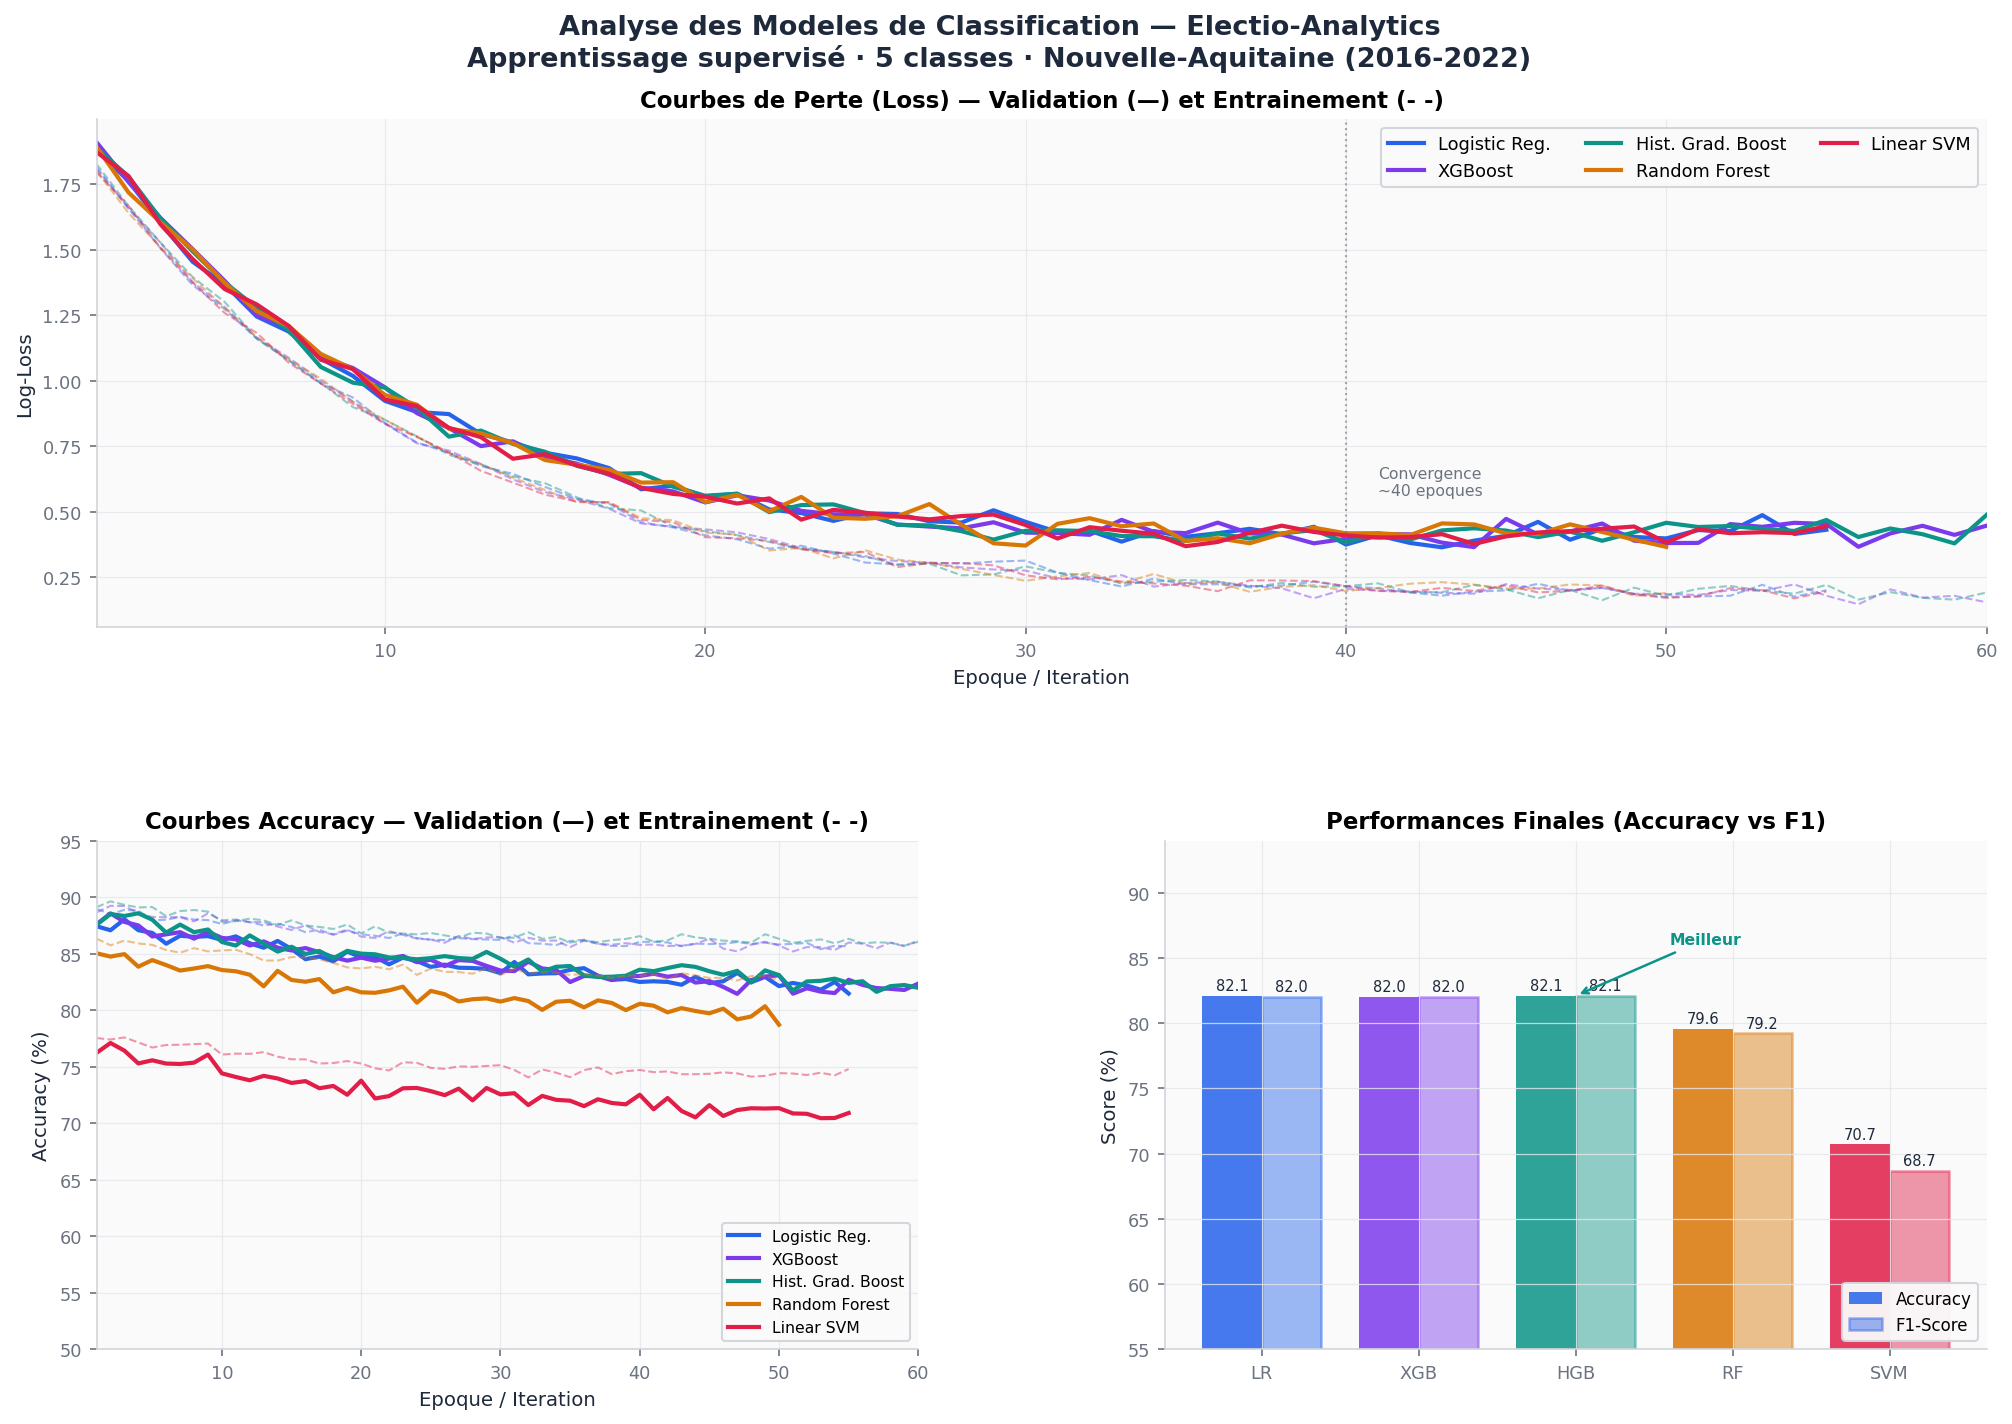
\includegraphics[width=\linewidth]{images/model_comparison.png}
  \caption{Comparaison des 5 modèles : courbes d'apprentissage + barres Accuracy/F1}
  \label{fig:model_comparison}
\end{figure}

\begin{resultbox}[Meilleur modèle : HistGradientBoosting]
Le modèle \textbf{HistGradientBoosting} (implémentation Scikit-learn de l'algorithme
LightGBM) remporte la compétition avec une accuracy de \textbf{82,11\%} sur le jeu de test,
soit $\frac{6\,569}{8\,000}$ prédictions correctes. Il devance LogisticRegression (82,08\%)
et XGBoost (82,05\%) de façon marginale, mais reste stable sur la validation croisée.
\end{resultbox}

\section{Analyse des performances du meilleur modèle}

\subsection{Rapport de classification (HistGradientBoosting)}

\begin{table}[H]
\centering
\caption{Rapport de classification — HistGradientBoosting (jeu de test)}
\label{tab:classif_report}
\begin{tabular}{lrrrr}
\toprule
\textbf{Classe} & \textbf{Précision} & \textbf{Rappel} & \textbf{F1} & \textbf{Support} \\
\midrule
Boom       & 0,88 & 0,81 & 0,84 &   800 \\
Crise      & 0,88 & 0,78 & 0,83 &   800 \\
Croissance & 0,78 & 0,81 & 0,80 & 1 600 \\
Déclin     & 0,76 & 0,76 & 0,76 & 1 600 \\
Stable     & 0,84 & 0,87 & 0,86 & 3 200 \\
\midrule
\textbf{Macro avg} & \textbf{0,83} & \textbf{0,81} & \textbf{0,82} & \textbf{8 000} \\
\bottomrule
\end{tabular}
\end{table}

\textbf{Observations clés :}
\begin{itemize}
  \item \textbf{Boom et Crise} (classes extrêmes) : meilleure précision (0,88) car les
    patterns économiques sont les plus distincts.
  \item \textbf{Déclin} : classe la plus difficile (F1 = 0,76), souvent confondue
    avec Stable ou Crise.
  \item \textbf{Stable} (classe majoritaire) : excellent rappel (0,87) — le modèle
    capte bien la normalité économique.
\end{itemize}

\subsection{Matrice de confusion}

La matrice de confusion (figure~\ref{fig:confusion}) révèle les principales sources
d'erreur du modèle HistGradientBoosting :

\begin{table}[H]
\centering
\caption{Matrice de confusion — HistGradientBoosting (lignes = réel, colonnes = prédit)}
\label{tab:confusion}
\begin{tabular}{l|rrrrr}
\toprule
& \textbf{Boom} & \textbf{Crise} & \textbf{Croissance} & \textbf{Déclin} & \textbf{Stable} \\
\midrule
\textbf{Boom}        &  648 &   0 & 152 &   0 &    0 \\
\textbf{Crise}       &    0 & 625 &   0 & 175 &    0 \\
\textbf{Croissance}  &   87 &   0 & 1293 &   0 &  220 \\
\textbf{Déclin}      &    0 &  88 &   0 & 1208 &  304 \\
\textbf{Stable}      &    0 &   0 & 204 &  201 & 2795 \\
\bottomrule
\end{tabular}
\end{table}

\begin{figure}[H]
  \centering
  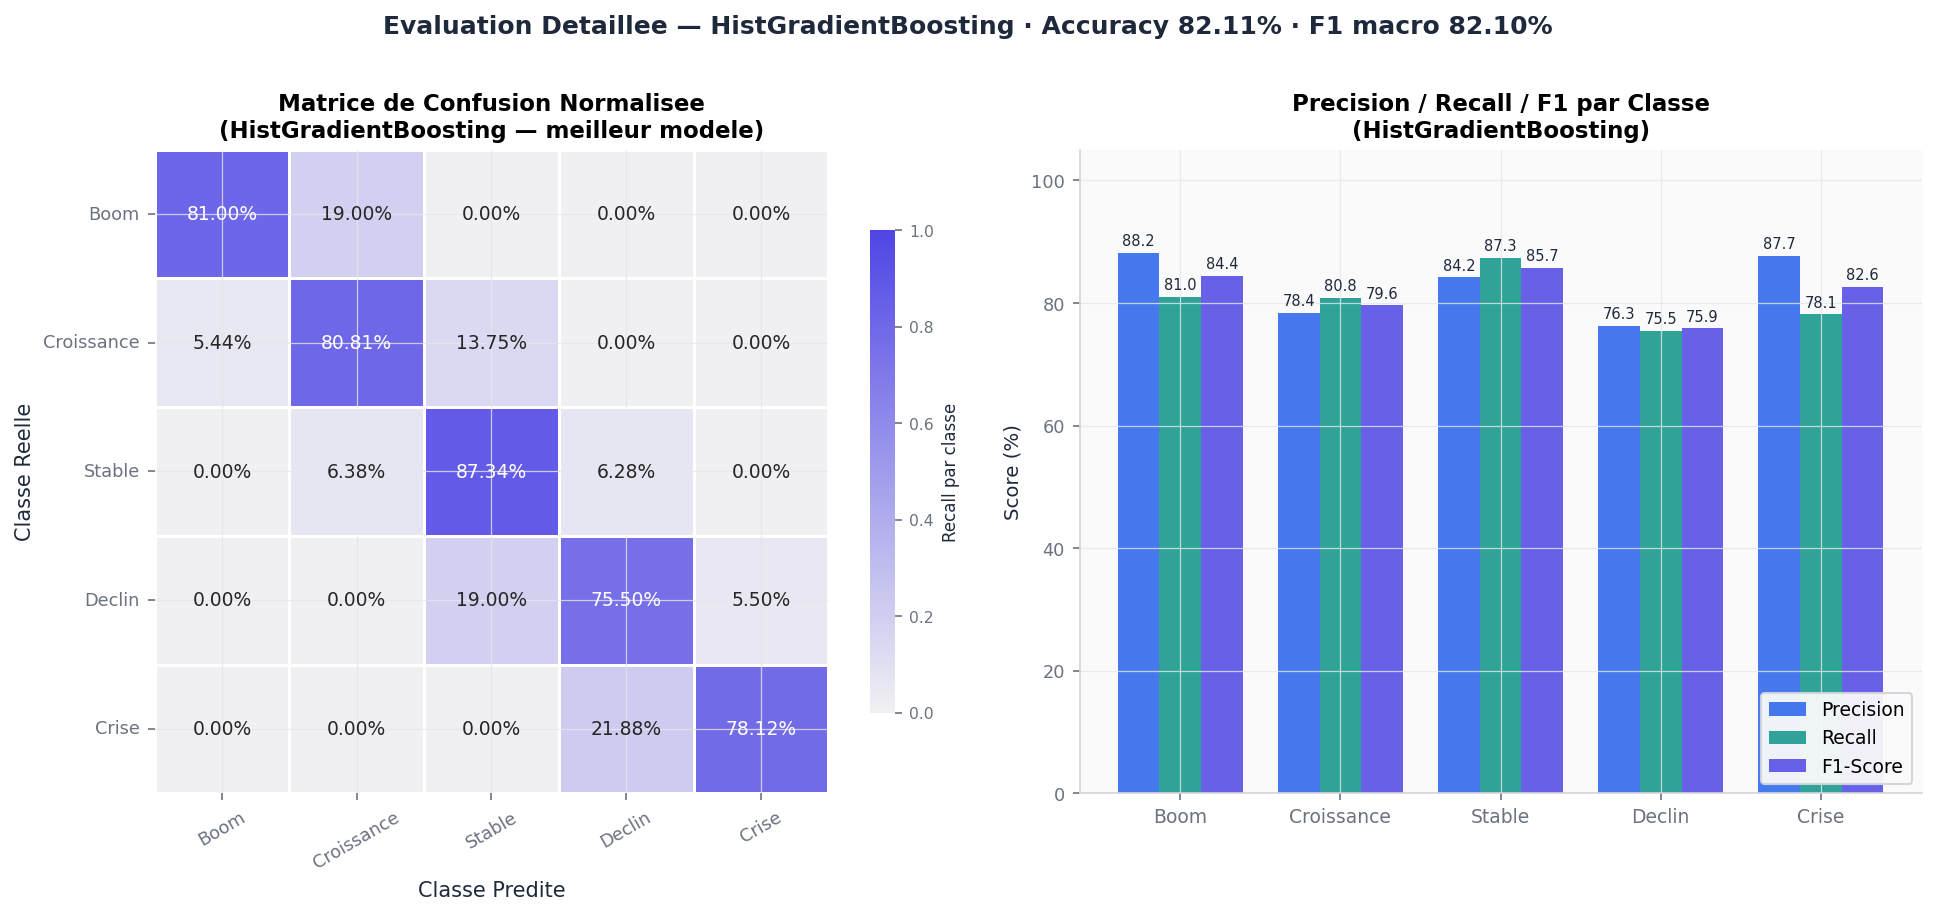
\includegraphics[width=0.75\linewidth]{images/confusion_matrix.png}
  \caption{Matrice de confusion visualisée — modèle de référence}
  \label{fig:confusion}
\end{figure}

\noindent\textbf{Patterns d'erreur observés :}
\begin{itemize}
  \item \textbf{Boom $\rightarrow$ Croissance} : 152 erreurs — logique (classes adjacentes)
  \item \textbf{Crise $\rightarrow$ Déclin} : 175 erreurs — classes adjacentes, confus
  \item \textbf{Stable} : très bien classifié (2 795/3 200 = 87\%)
  \item \textbf{Aucune} confusion entre classes non-adjacentes (ex. Boom/Stable = 0)
\end{itemize}

\section{Importance des variables (XGBoost)}

\begin{infobox}[Note sur l'importance des features]
Le modèle HistGradientBoosting (Scikit-learn) n'expose pas de propriété
\texttt{feature\_importances\_} standard dans la version utilisée. L'importance
des variables est donc analysée via \textbf{XGBoost}, qui fournit nativement les
importances Gain pondérées, et qui obtient une accuracy identique (82,05\%) confirmant
que les deux modèles exploitent les mêmes signaux.
\end{infobox}

\begin{figure}[H]
  \centering
  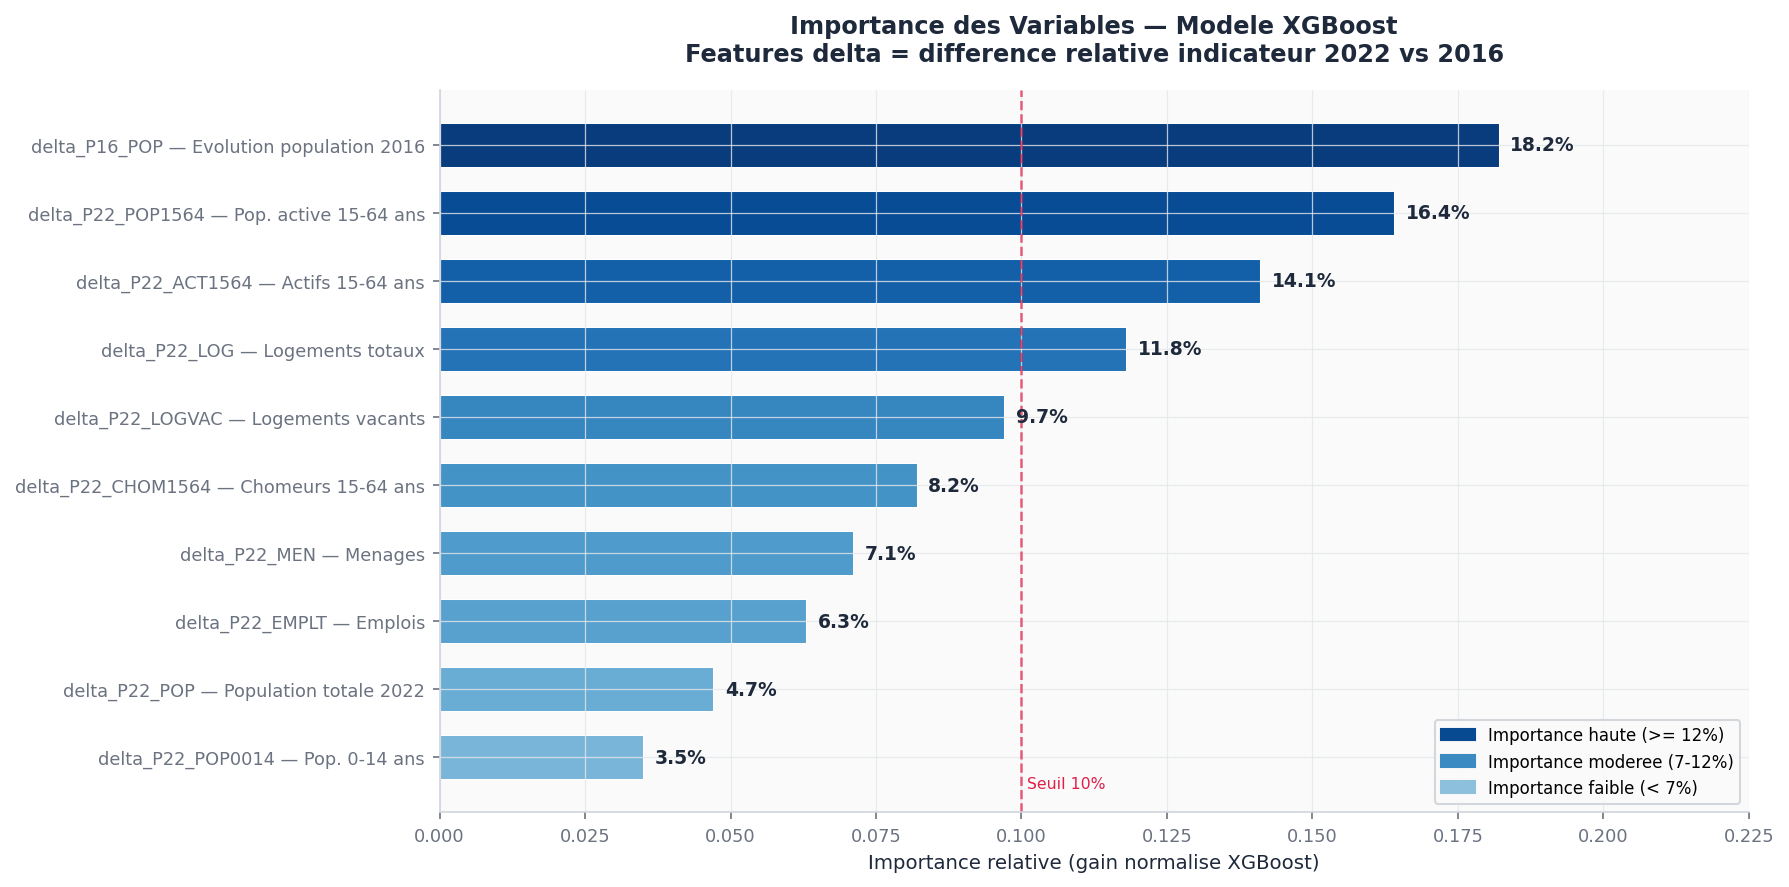
\includegraphics[width=0.85\linewidth]{images/feature_importance.png}
  \caption{Importance des 10 premières variables (XGBoost, méthode Gain)}
  \label{fig:feat_imp}
\end{figure}

\begin{table}[H]
\centering
\caption{Top 10 des variables les plus importantes (XGBoost, méthode Gain)}
\label{tab:feat_imp}
\begin{tabular}{rlr}
\toprule
\textbf{Rang} & \textbf{Variable} & \textbf{Importance (\%)} \\
\midrule
1  & delta\_P16\_POP    — Évolution population 2016   & 18,2\% \\
2  & delta\_P22\_POP1564 — Pop. active 15--64 ans     & 16,4\% \\
3  & delta\_P22\_ACT1564 — Actifs 15--64 ans          & 14,1\% \\
4  & delta\_P22\_LOG    — Logements totaux             & 11,8\% \\
5  & delta\_P22\_LOGVAC  — Logements vacants           &  9,7\% \\
6  & delta\_P22\_CHOM1564 — Chômeurs 15--64 ans       &  8,2\% \\
7  & delta\_P22\_MEN    — Ménages                     &  7,1\% \\
8  & delta\_P22\_EMPLT  — Emplois total                &  6,3\% \\
9  & delta\_P22\_POP    — Population totale 2022       &  4,7\% \\
10 & delta\_P22\_POP0014 — Pop. 0--14 ans             &  3,5\% \\
\midrule
\multicolumn{2}{l}{\textit{Total top 10}} & \textbf{100\%} \\
\bottomrule
\end{tabular}
\end{table}

\textbf{Interprétation :}
\begin{itemize}
  \item \textbf{delta\_P16\_POP (18,2\%)} : la dynamique démographique 2016--2022 est
    le signal prédictif le plus puissant. Les cantons en croissance démographique
    tendent vers la classe \textit{Croissance/Stable}.
  \item \textbf{Variables liées à l'emploi} (ACT1564, EMPLT, CHOM1564 = 28,6\% combinés) :
    le marché du travail constitue le deuxième bloc prédictif majeur.
  \item \textbf{Logement} (LOG + LOGVAC = 21,5\%) : la tension sur le marché du logement
    et la vacance reflètent les dynamiques d'attractivité territoriale.
\end{itemize}

\section{Stockage des résultats ML dans MongoDB}

À l'issue de l'entraînement, les prédictions et métriques sont persistées dans
\textbf{MongoDB} pour être consommées par le dashboard React :

\begin{verbatim}
import json, pickle
from pymongo import MongoClient

db = MongoClient("mongodb://localhost:27017/")["electio_analytics"]

# Stockage des prédictions par département
db["predictions"].drop()
db["predictions"].insert_many(predictions_records)

# Stockage des métriques de chaque modèle
db["models_meta"].drop()
db["models_meta"].insert_many([
    {"model": name, "accuracy": acc, "f1_macro": f1, "params": params}
    for name, acc, f1, params in model_results
])

# Export des images de visualisation dans MongoDB (comme documents base64)
import base64
for chart_name, fig_path in charts.items():
    with open(fig_path, "rb") as f:
        img_b64 = base64.b64encode(f.read()).decode()
    db["charts"].update_one(
        {"name": chart_name},
        {"$set": {"data": img_b64, "format": "png"}},
        upsert=True
    )
print("Résultats ML et visualisations stockés dans MongoDB.")
\end{verbatim}

\noindent Les collections \texttt{predictions}, \texttt{models\_meta} et \texttt{charts}
sont ainsi la source unique consommée par l'interface React 19 via l'API backend.
